\begin{center}
	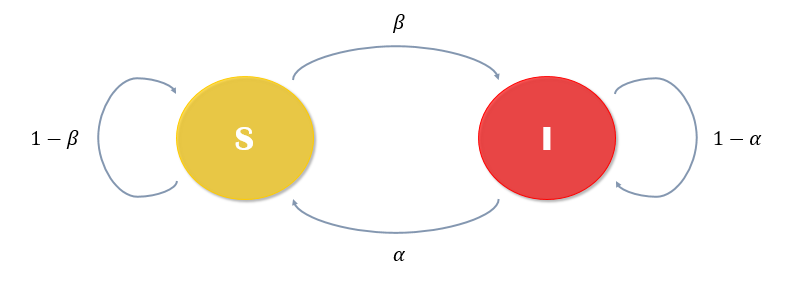
\includegraphics[width=0.65\linewidth]{Imagenes/esquema_sis.PNG}
\end{center}

\begin{center}
    \caption{Fuente: Jorge Ibañez 2021} \\
\end{center}

De donde se obtiene el siguiente sistema de ecuaciones diferenciales:
\begin{equation}
    \left\{
    \begin{array}{c}
        S' = \alpha I - \beta SI \\
        I' = \beta SI - \alpha I
    \end{array}
    \right. \label{eq:1}
\end{equation}

Para modelar el comportamiento de los individuos mediante el sistema de ecuaciones diferenciales descrito en \ref{eq:1}, se consideran los contactos entre las poblaciones de susceptibles e infectados a partir del producto de las variables S e I. 

El término $\alpha I$ indica la probabilidad de que un individuo se recupere mientras que el término $\beta SI$ indica la probabilidad de que un individuo susceptible se infecte al de tener contacto con un individuo infectado. \cite{diego2010}

\subsection*{El modelo SIR}

A diferencia del modelo SIS, el modelo SIR describe las interacciones entre los estados susceptible (S), infectado (I) y recuperado (R). Es posible que un individuo susceptible adquiera el virus y que posteriormente pueda recuperarse, sin embargo en este modelo no es posible que un individuo que no ha tenido la enfermedad en algún momento se cure de esta, para comprender de una mejor manera el funcionamiento del modelo $SIR$ observemos el siguiente diagrama:

\begin{center}
	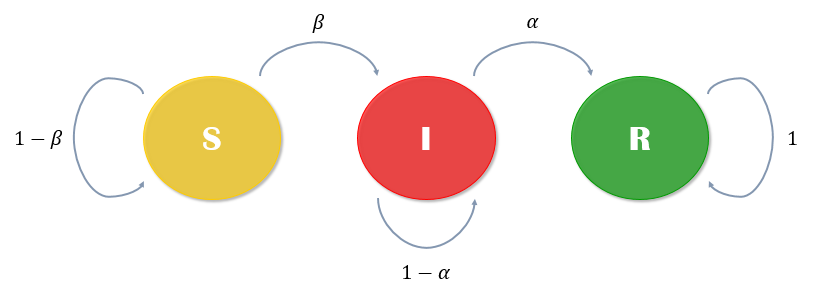
\includegraphics[width=0.7\textwidth]{Imagenes/esquema_sir.PNG}
\end{center}
\begin{center}
    \caption{Fuente: Jorge Ibañez 2021}
\end{center}

Al igual que en el caso del modelo $SIS$, las constantes $\alpha$ y $\beta$ representan las tasas de recuperación e infección respectivamente; una vez dicho esto podemos describir el modelo $SIR$ en ecuaciones diferenciales:
\begin{equation}
    \left\{
    \begin{array}{l}
        S' = -\beta SI \\
        I' = \beta SI-\alpha I \\
        R' = \alpha I
    \end{array}
    \right.\label{equ3}
\end{equation}
